\section{Istruzione per l'utilizzo}
  L'header della {dashboard}\ped{G} è uguale come struttura per ogni tipo di utente. Su di esso troviamo un link che porta alla modifica dei dati personali, chiamato \textit{Profilo} e un link \textit{Esci}, che, se cliccato, effettua il logout dal sistema.



\subsection{Interfaccia}
    \begin{figure}[H]
        \centering
        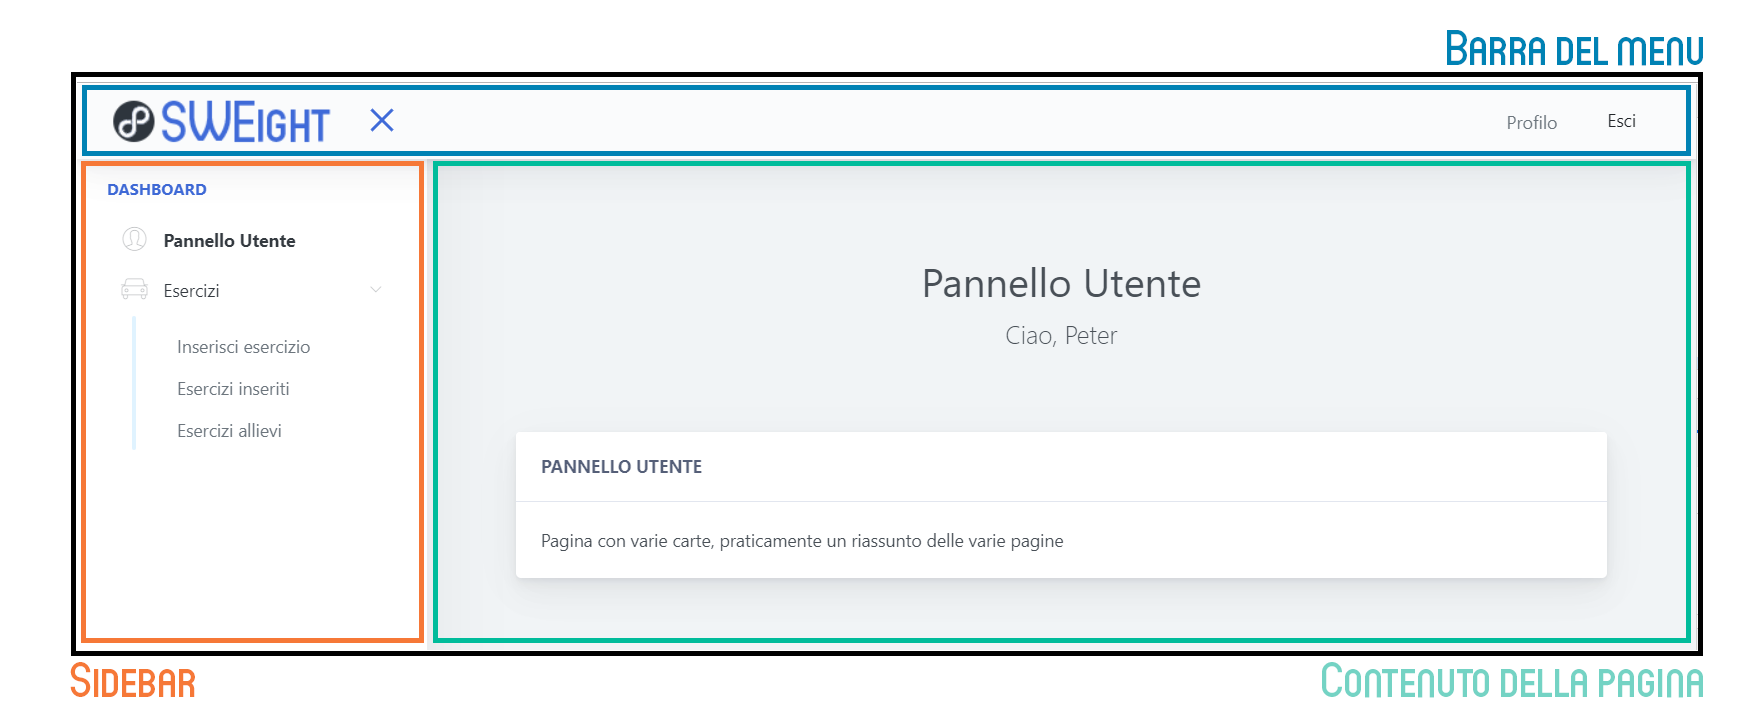
\includegraphics[width=17cm]{sez/img/istruzioni/dashboardMod.png} 
        \caption{Panoramica dell'interfaccia}\label{fig:1}
    \end{figure}
  Questa sezione serve per definire i termini con cui chiamare gli elementi che compongono la pagina dell'applicazione.
    Componenti principali:
    \begin{itemize}
        \item Barra del menu;
        \item {Sidebar}\ped{G};
        \item Contenuto della pagina.
    \end{itemize}


\subsection{Utente non autenticato}
    \subsubsection{Registrazione}
    	\begin{figure}[H]
        	\centering
        	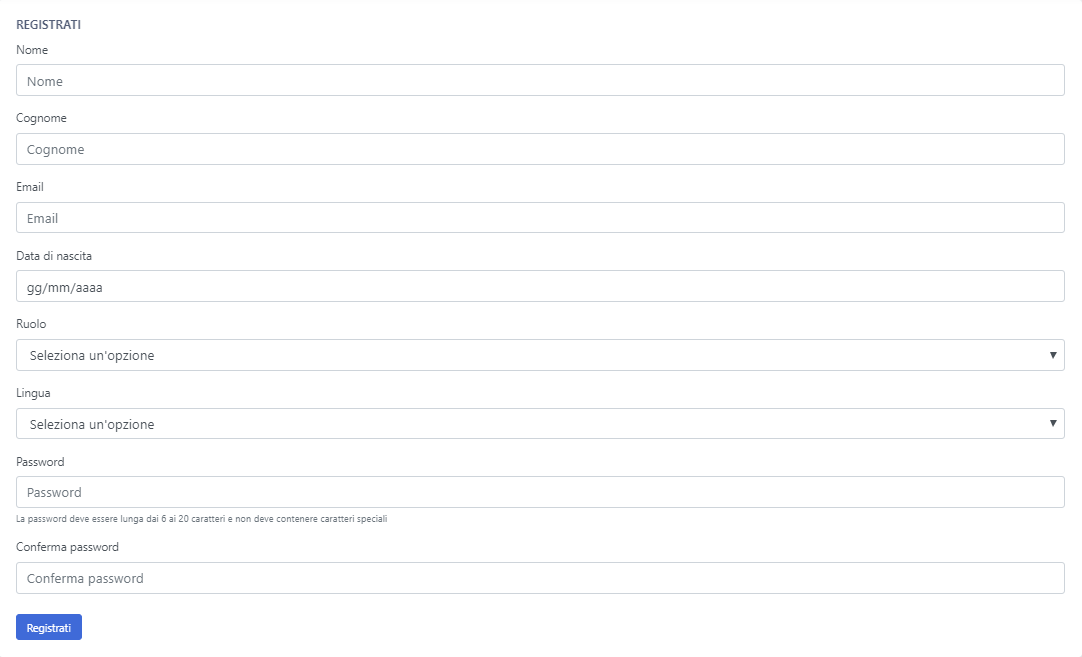
\includegraphics[width=1\linewidth]{sez/img/autenticazione/formRegistrazione.PNG} 
        	\caption{Form per la registrazione}\label{fig:registrazione}
    	\end{figure}
	  Se non si è ancora registrati è possibile farlo cliccando sul bottone \textit{Registrati} presente nella barra del menu. Una volta compilato il form sarà possibile accedere alla piattaforma come utente autenticato. Se si sceglie come ruolo \textit{sviluppatore} sarà necessario attendere una conferma da parte dell'amministratore prima di poter accedere. I dati sono tutti obbligatori e il form visualizzato sarà quello in \autoref{fig:registrazione}.

    \subsubsection{Login}
    	\begin{figure}[H]
        	\centering
        	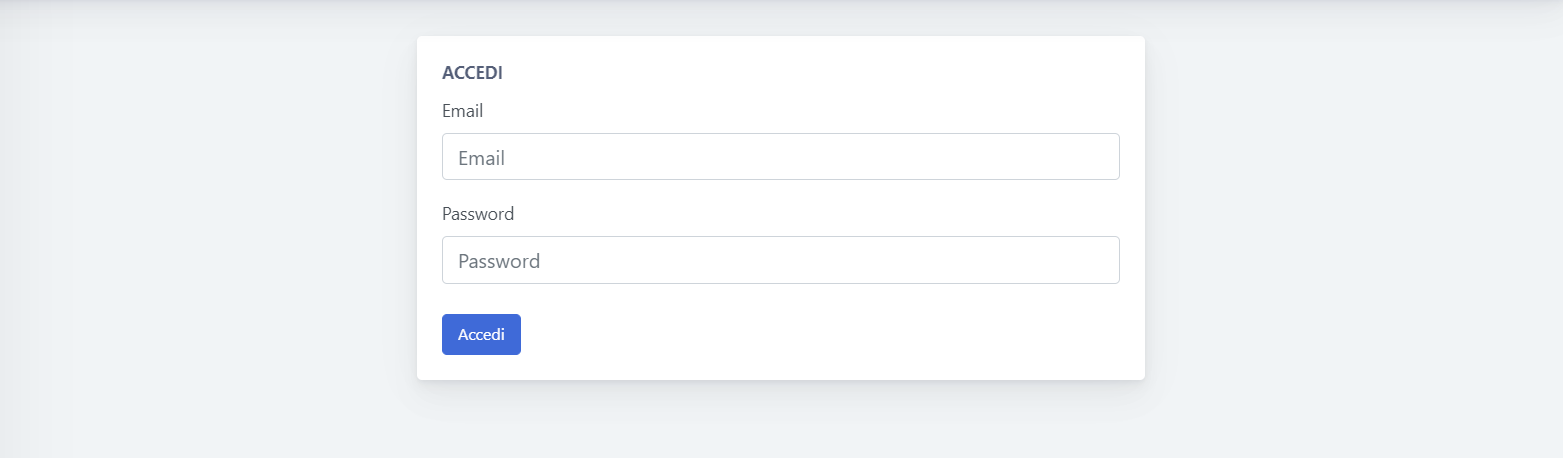
\includegraphics[width=1\linewidth]{sez/img/autenticazione/formAccedi.PNG} 
        	\caption{Dati per effettuare l'accesso}\label{fig:1}
    	\end{figure}
 	  Dopo aver effettuato la registrazione si accede cliccando su \textit{Accedi} nella barra del menu. Si accede inserendo email e password.


% UTENTE AUTENTICATO
\subsection{Utente autenticato generico}

    \subsubsection{Logout}
    Per effettuare il {logout}\ped{G} si deve cliccare sulla voce \textit{Esci} dalla barra del menu. Facendo ciò, l'utente termina la propria sessione.

    \subsection{Studente}
      Lo studente può svolgere esercizi, che vengono corretti tramite soluzione automatiche o soluzioni di un'insegnante.
        \subsubsection{Sidebar}
          La sidebar dello studente presenta le seguenti voci:
            \begin{itemize}
                \item Pannello utente;
                \item Esercitazione libera;
                \item Compiti per casa;
                \item Esercizi svolti.
            \end{itemize}
            
            
            
            
            
            
        \subsubsection{Pannello utente}
          Il pannello utente è un riassunto di tutti i progressi e le attività svolte dallo studente.
          Contenuto presente all'interno della pagina:
        	\begin{itemize}
        		\item Progressi;
        		\item Traguardi;
        		\item Traguardo corrente;
        		\item Prossimo traguardo;
        		\item Valutazioni;
        		\item Esercizi recenti;
        		\item Insegnanti preferiti.
        	\end{itemize}
        
        
               
	\newpage
        \subsubsection{Esercitazione libera}      
        	\begin{figure}[H]
                \centering
                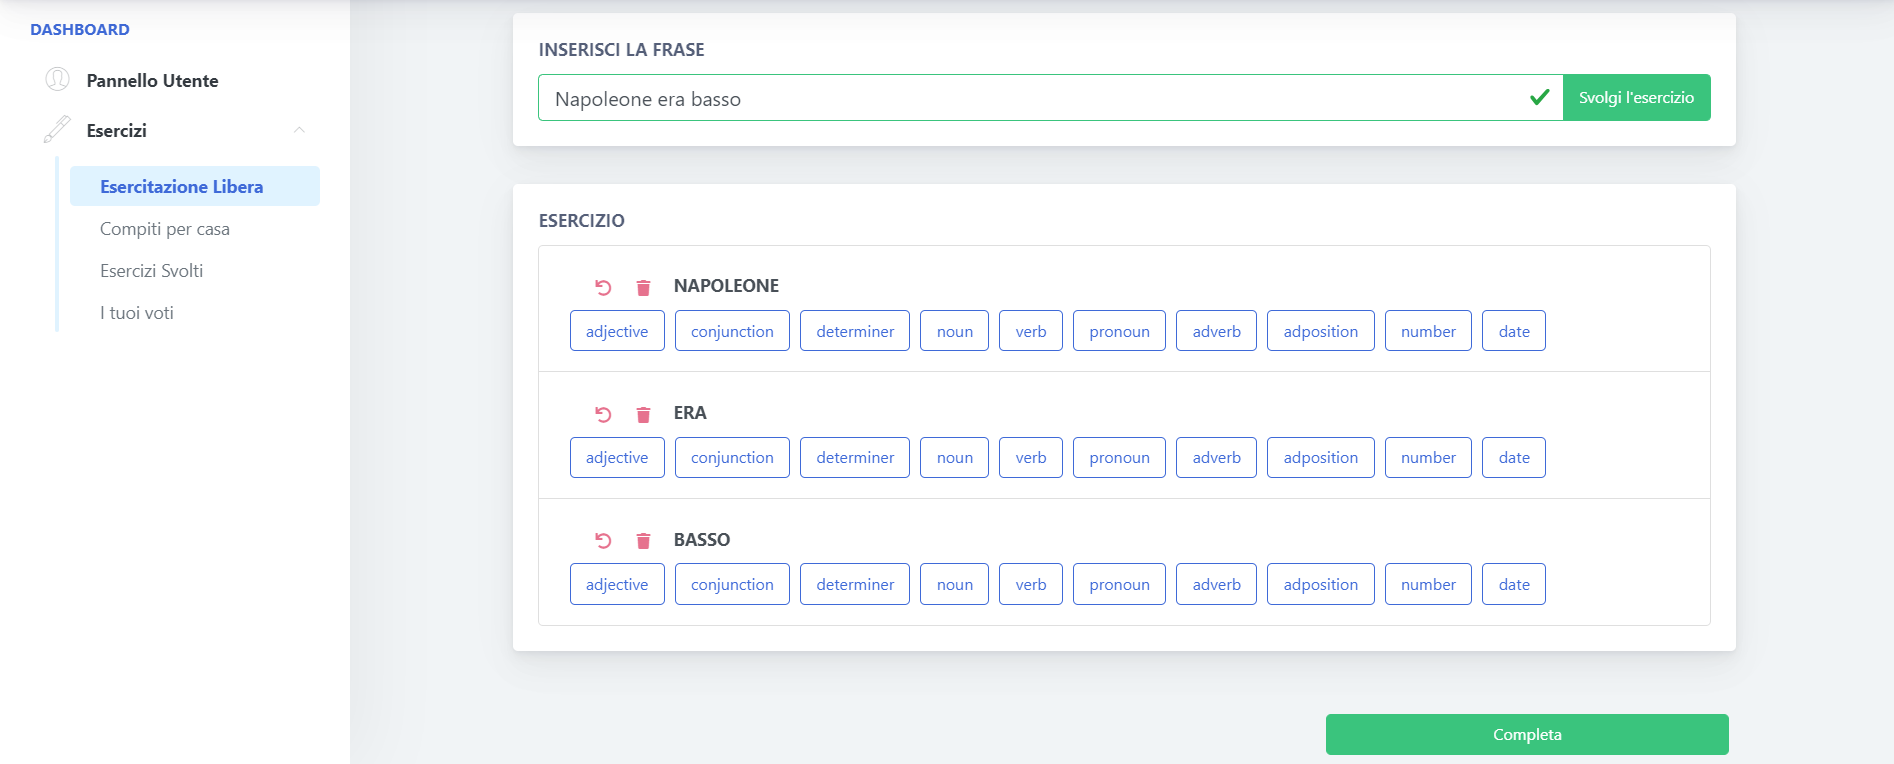
\includegraphics[width=17cm]{sez/img/studente/esercitazioneLiberaEsegui.PNG} 
                \caption{Svolgimento esercizio libero}\label{fig:1}
        	\end{figure}
          In questa pagina è possibile svolgere un esercizio inserendo nel form una frase da analizzare.
          Se la frase non è stata inserita da nessun insegnante la 
        correzione sarà generata automaticamente.
        \\ Svolgimento:
        	\begin{enumerate}        
            	\item Scrivere la frase da analizzare dentro al form;
            	\item Cliccare su \textit{Svolgi l'esercizio};
            	\item Svolgere l'esercizio e cliccare \textit{Completa}.
        	\end{enumerate}

      
        \newpage
  		\subsubsection{Compiti per casa}
 		  In questa sezione è possibile visualizzare gli esercizi che sono stati assegnati dall'insegnante. Lo studente può scegliere uno qualsiasi fra gli esercizi elencati.
        	\begin{figure}[H]
            	\centering
            	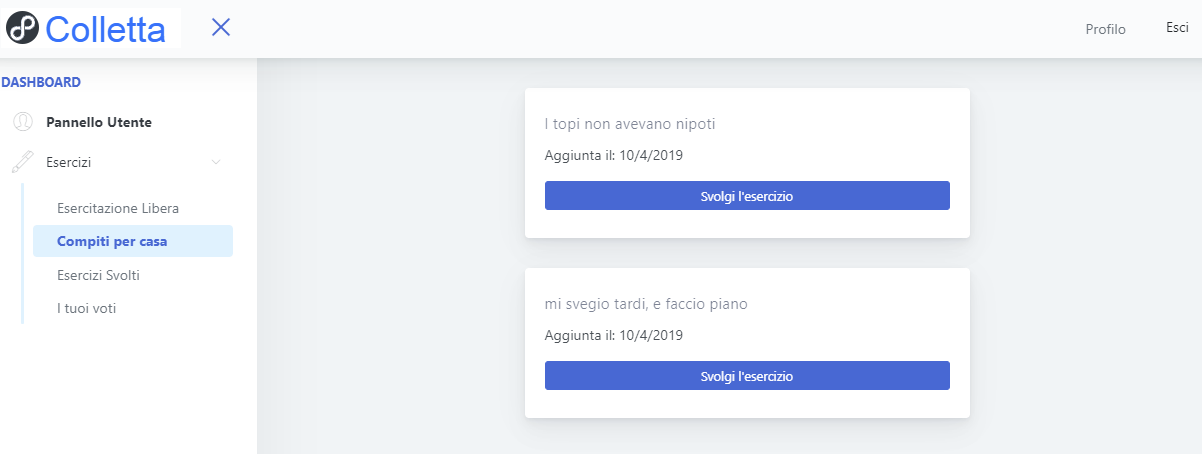
\includegraphics[width=17cm]{sez/img/studente/compitopercasa.PNG} 
            	\caption{Scelta esercizio da risolvere}\label{fig:1}
        	\end{figure}

		  Lo studente sceglie l'esercizio da svolgere tra quelli che sono stati assegnati cliccando su \textit{Svolgi l'esercizio}.   
       
        	\begin{figure}[H]
            	\centering
            	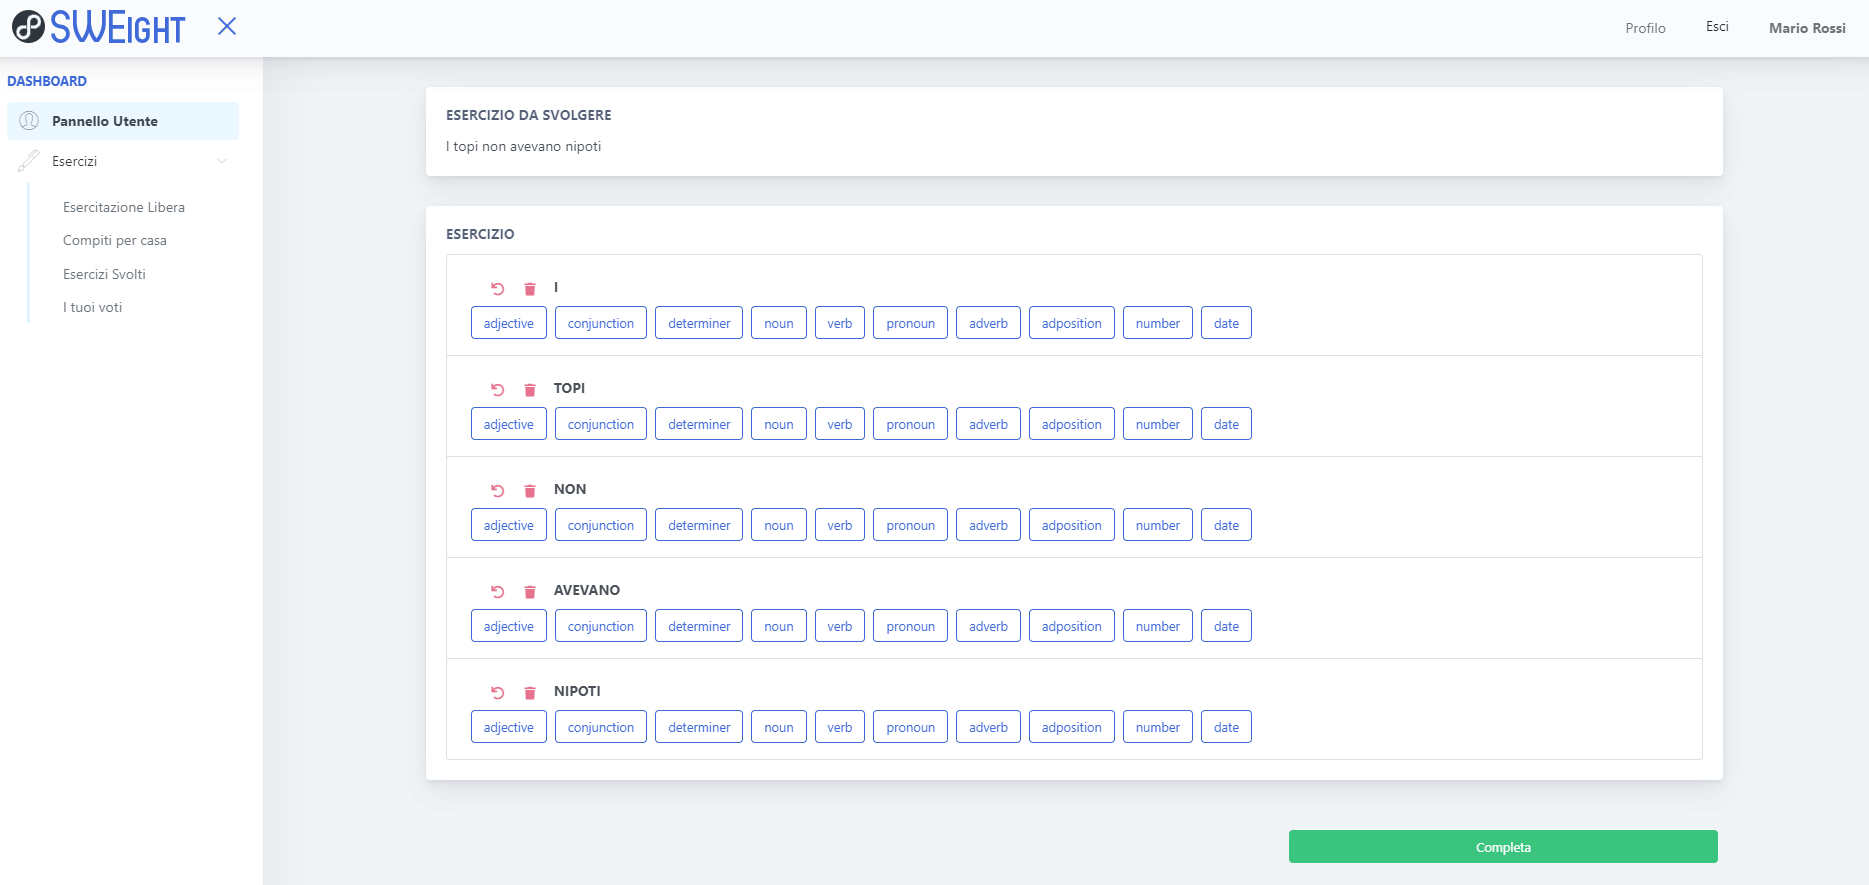
\includegraphics[width=17cm]{sez/img/studente/svolgimentoesercizio.PNG} 
            	\caption{Svolgimento esercizio}\label{fig:1}
        	\end{figure}      
          Lo studente analizza ogni parola tramite dei bottoni che lo guidano per le scelte. Per ogni parola è possibile tornare indietro di un passo o resettare l'intera soluzione. Infine, cliccando \textit{Completa}, lo studente invia la sua soluzione che verrà confrontata e valutata contro quella dell'insegnate.
        
        
        
        
        \subsubsection{Esercizi svolti}
        	\begin{figure}[H]
            	\centering
            	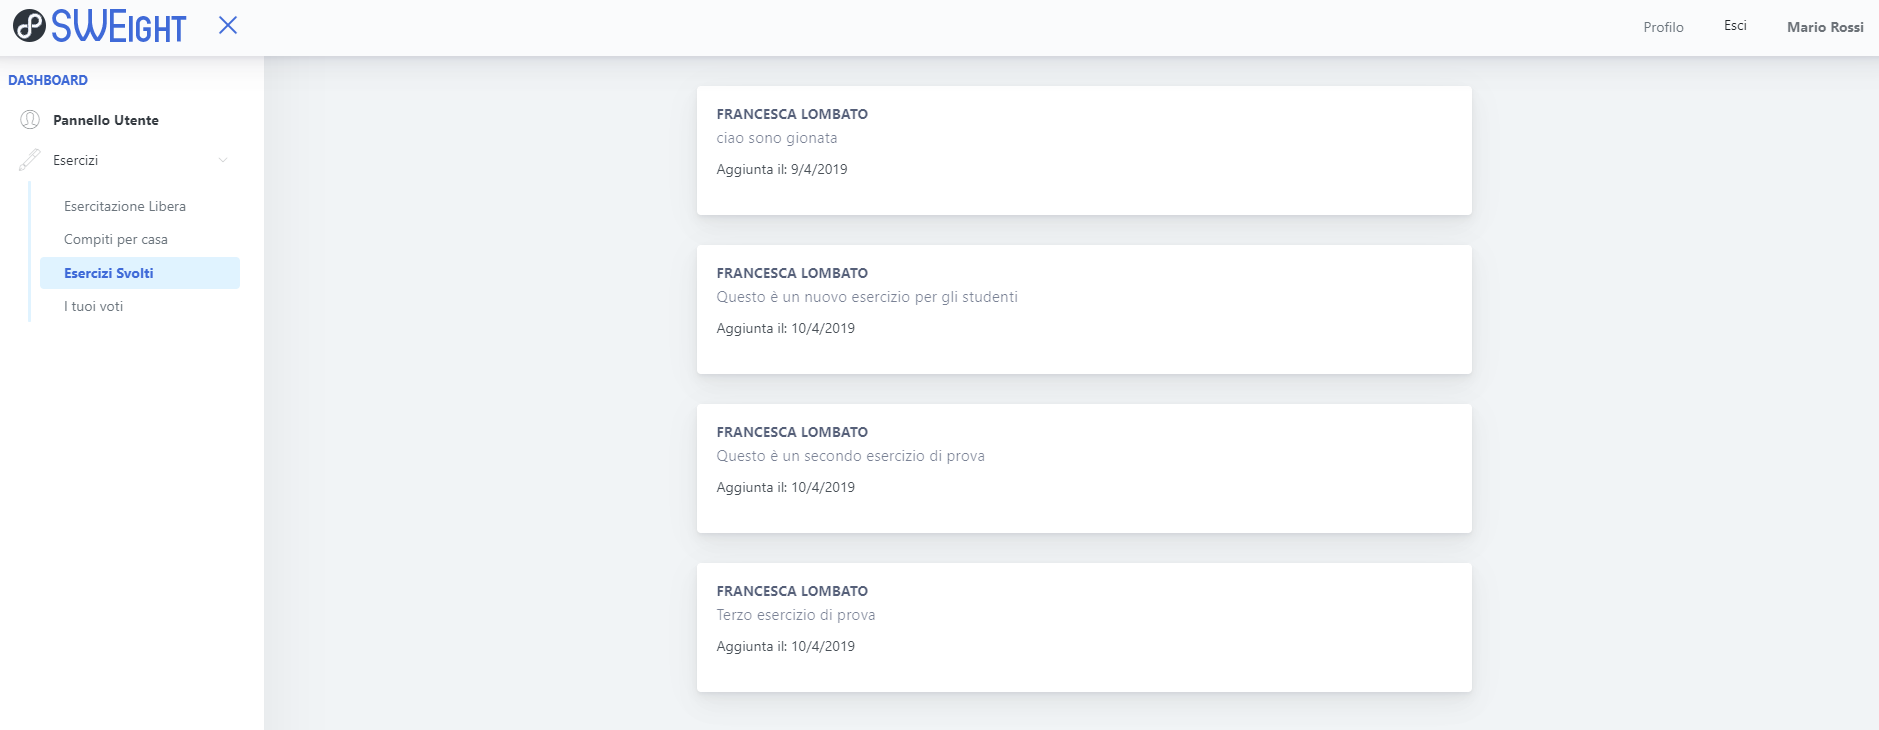
\includegraphics[width=17cm]{sez/img/studente/esercizisvolti.PNG} 
            	\caption{Storico esercizi svolti}\label{fig:1}
        	\end{figure}
          In questa pagina è possibile visualizzare lo storico degli esercizi che sono stati svolti.
        
\newpage
    \subsection{Insegnante}
      L'insegnante è l'utente che può inserire esercizi e assegnarli.
        \subsubsection{Sidebar}
          La sidebar dell'insegnante presenta le seguenti voci:
        	\begin{itemize}
            	\item Pannello utente;
            	\item Inserisci esercizio;
            	\item Esercizi inseriti;
            	\item Esercizi allievi.
        	\end{itemize}
        
        
        
        \subsubsection{Pannello utente}
          Il pannello utente è un riassunto di tutti i progressi e le attività.
         \\Contenuto presente all'interno della pagina:
        	\begin{itemize}
        		\item Storico esercizi inseriti; 
        		\item Esercizi recenti svolti dagli studenti;
        		\item Elenco propri studenti;
        		\item Elenco classi studenti.
        	\end{itemize}
        
        
        
        
        \subsubsection{Inserisci esercizio}
          Questa sezione da la possibilità all'insegnante di inserire un esercizio.
        	\begin{figure}[H]
            	\centering
        		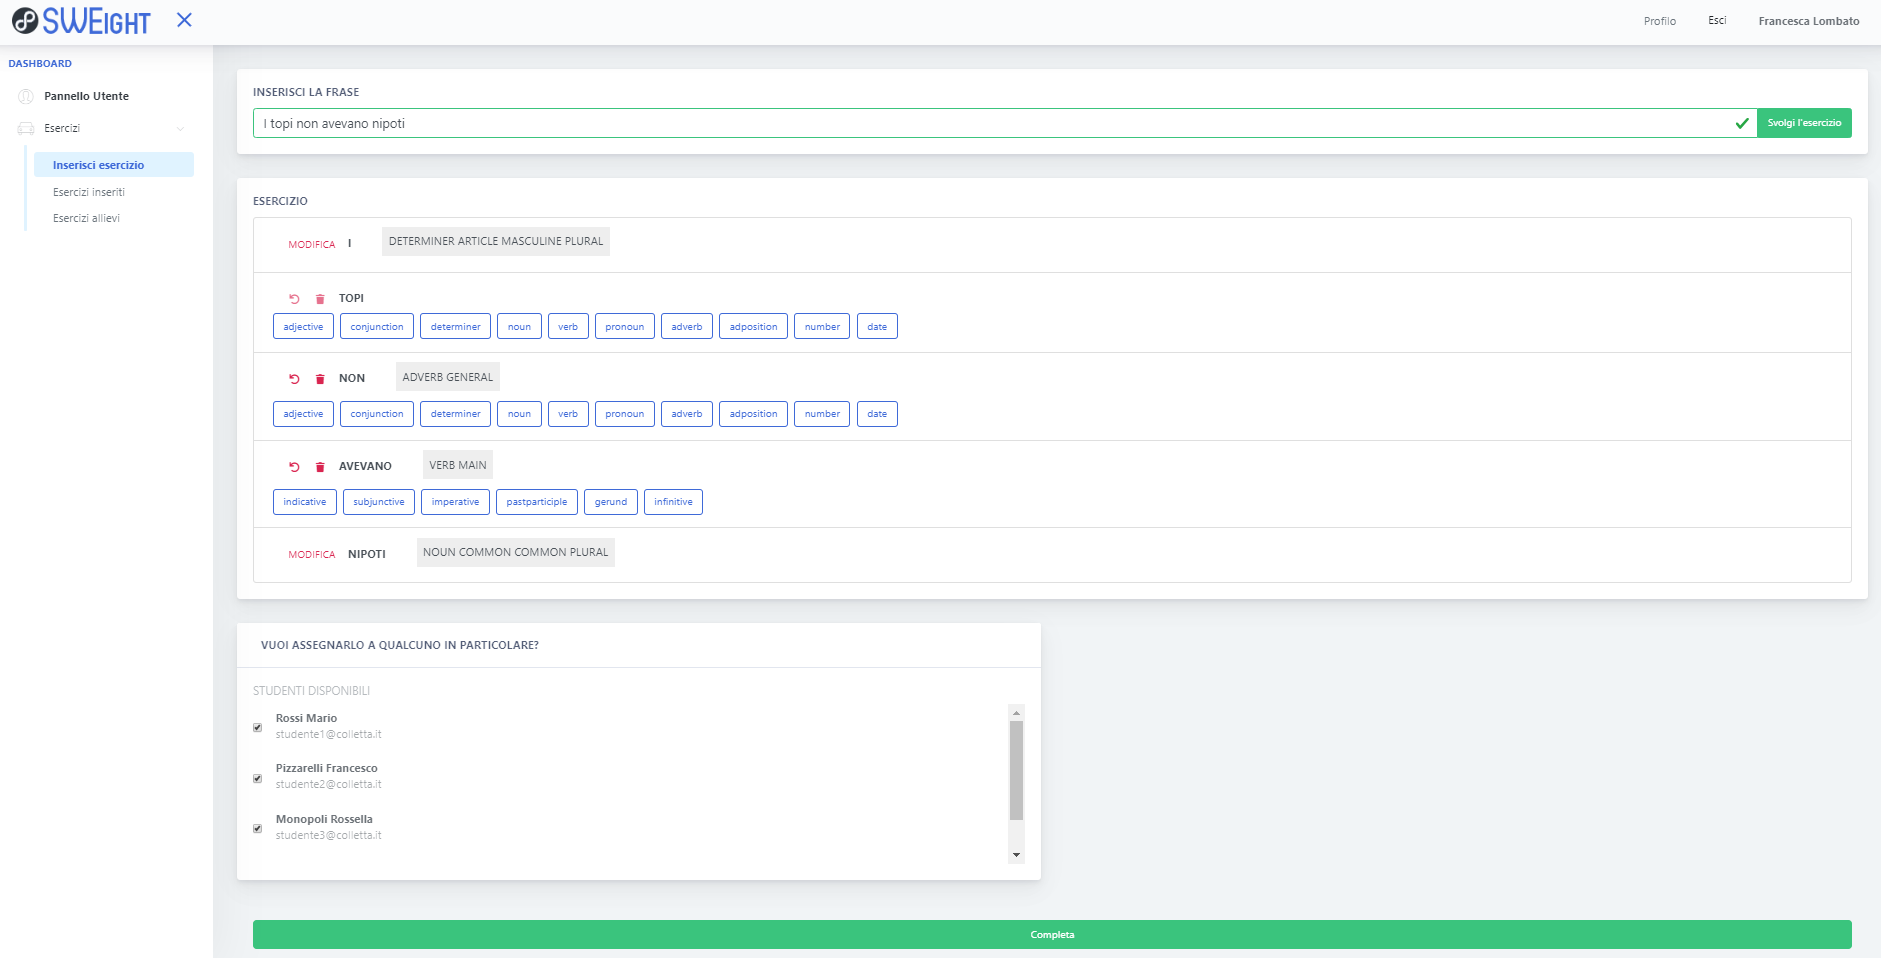
\includegraphics[width=17cm]{sez/img/insegnante/inserisciEsercizio.PNG} 
            	\caption{Inserimento e assegnazione esercizio}\label{fig:1}
        	\end{figure}
        
          Dopo aver inserito la frase, verrà visualizzata la correzione automatica. Se ritenuta errata c'è la possibilità di modificare la soluzione cliccando su \textit{Modifica}. Durante lo svolgimento dell'esercizio l'insegnante ha la possibilità di tornare indietro di un passo, o di resettare completamente la soluzione per ogni parola. Finita la correzione, l'insegnate ha la possibilità di assegnare l'esercizio a uno studente e cliccando \textit{Completa} esso verrà aggiunto nel database.
        
        
        
        \subsubsection{Esercizi inseriti}
        Questa sezione permette di visualizzare tutti gli esercizi inseriti.
        
        
        
        
        \subsubsection{Esercizi allievi}        
          In questa sezione sono visibili i risultati ottenuti dagli allievi dell'insegnante.
        
        
        
        
	\newpage
    \subsection{Sviluppatore}
    
    	\subsubsection{Sidebar} 
    	  La sidebar dello sviluppatore presenta le seguenti voci:
    		\begin{itemize}
    			\item Pannello utente;
    			\item Pannello sviluppatore.
    		\end{itemize}
    
    
    
    
    	\subsubsection{Pannello utente}
    	  Contenuto presente all'interno della pagina:
        	\begin{itemize} 
        		\item Messaggio di benvenuto.
        	\end{itemize}




    	\subsubsection{Pannello sviluppatore}
    		\begin{figure}[H]
				\centering
				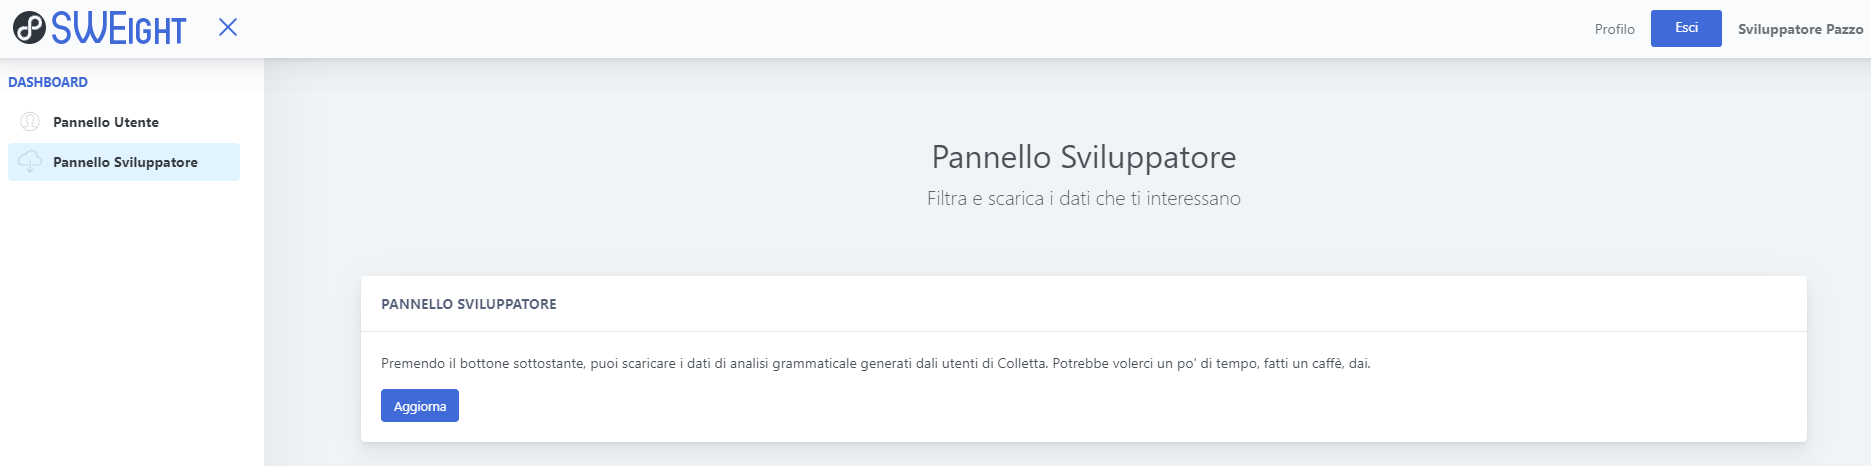
\includegraphics[width=17cm]{sez/img/sviluppatore/datipronti.PNG}
				\caption{Scaricamento dati disponibili}\label{fig:1}
			\end{figure}
		  Cliccando sul bottone di scaricamento, lo sviluppatore può scaricare i dati prodotti dagli utenti.




	\newpage
	\subsection{Amministratore}
		\subsubsection{Sidebar}
		  Voci di menu:
			\begin{itemize}
				\item Pannello utente;
				\item Sviluppatori;
				\item Utenti.
			\end{itemize}



		\subsubsection{Pannello utente}
		 Contenuto del pannello utente:
			\begin{itemize}
				\item Messaggio di benvenuto.
			\end{itemize}




		\subsubsection{Sviluppatori}
			\begin{figure}[H]
				\centering
				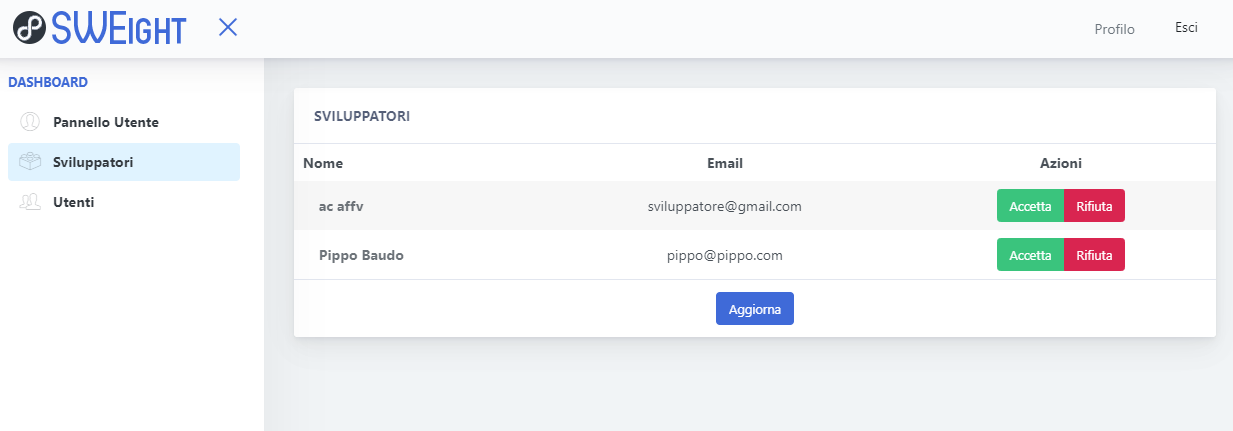
\includegraphics[width=17cm]{sez/img/amministratore/conf_ric_svil.PNG}
				\caption{Richieste di iscrizione degli sviluppatori}\label{fig:1}
			\end{figure}
		  In questa pagina l'amministratore può approvare o rifiutare le richieste di iscrizione degli sviluppatori.


		\subsubsection{Utenti}
			\begin{figure}[H]
				\centering
				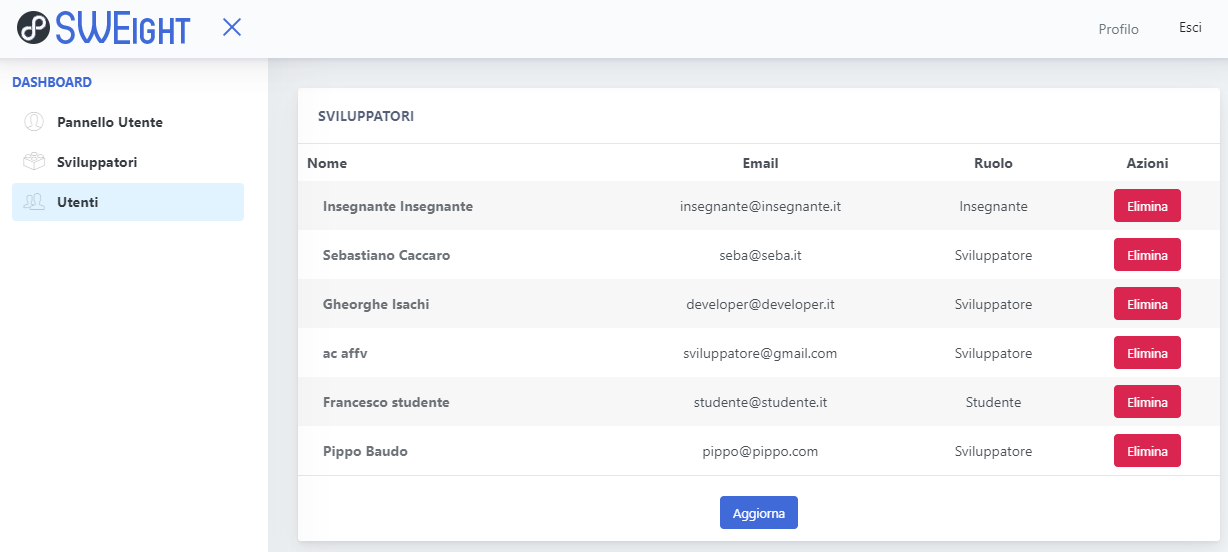
\includegraphics[width=17cm]{sez/img/amministratore/gestisciutenti.PNG}
				\caption{Gestione utenti}\label{fig:1}
			\end{figure}
		  In questa pagina l'amministratore può visualizzare gli utenti iscritti ed eventualmente eliminarli dal sito.
